% ---------------------------------------------------------------------------------------------------------------
% TEMPLATE PARA TRABALHO DE CONCLUSÃO DE CURSO
% Universidade Tecnológica Federal do Paraná - UTFPR
% Customização da classe abnTeX2 (http://www.abntex.net.br/) para as normas da UTFPR
%
% Projeto: http://tcc.tsi.gp.utfpr.edu.br/paginas/modelos-latex-da-utfpr
% Autores: Diego Marczal
% 	       Michael Vornes <https://github.com/mvornes>
%
%----------------------------------------------------------------------------------------------------------------
 % Codificação: UTF-8
% LaTeX:  abnTeX2
% ---------------------------------------------------------------------------------------------------------------


% CARREGA CLASSE PERSONALIZADA DA UNOPAR--------------------------------------------------------------------------
\documentclass[%twoside,                   	% Impressão em frente e verso
    	        oneside,                   		% Impressão apenas frente
]{configuracoes/unopar-abntex2}


% INCLUI ARQUIVOS DE CONFIGURAÇÕES-------------------------------------------------------------------------------
% REFERÊNCIAS------------------------------------------------------------------
\usepackage[%
    alf,
    abnt-emphasize=bf,
    bibjustif,
    recuo=0cm,
    abnt-url-package=url,       % Utiliza o pacote url
    abnt-refinfo=yes,           % Utiliza o estilo bibliográfico abnt-refinfo
    abnt-etal-cite=3,
    abnt-etal-list=3,
    abnt-thesis-year=final
]{abntex2cite}                  % Configura as citações bibliográficas conforme a norma ABNT

% PACOTES----------------------------------------------------------------------
\usepackage[utf8]{inputenc}                                 % Codificação do documento
\usepackage[T1]{fontenc}                                    % Seleção de código de fonte
\usepackage{booktabs}                                       % Réguas horizontais em tabelas
\usepackage{color, colortbl}                                % Controle das cores
\usepackage{float}                                          % Necessário para tabelas/figuras em ambiente multi-colunas
\usepackage{graphicx}                                       % Inclusão de gráficos e figuras
% \usepackage{icomma}                                         % Uso de vírgulas em expressões matemáticas
\usepackage{indentfirst}                                    % Indenta o primeiro parágrafo de cada seção
\usepackage{microtype}                                      % Melhora a justificação do documento
% \usepackage{multirow, array}                                % Permite tabelas com múltiplas linhas e colunas
% \usepackage{subeqnarray}                                    % Permite subnumeração de equações
% \usepackage{lastpage}                                       % Para encontrar última página do documento
\usepackage{verbatim}                                       % Permite apresentar texto tal como escrito no documento, ainda que sejam comandos Latex
\usepackage{amsfonts, amssymb, amsmath}                     % Fontes e símbolos matemáticos
% \usepackage[algoruled, portuguese]{algorithm2e}             % Permite escrever algoritmos em português
%\usepackage[scaled]{helvet}                                % Usa a fonte Helvetica
\usepackage{times}                                          % Usa a fonte Times
%\usepackage{palatino}                                      % Usa a fonte Palatino
%\usepackage{lmodern}                                       % Usa a fonte Latin Modern
% \usepackage[bottom]{footmisc}                               % Mantém as notas de rodapé sempre na mesma posição
\usepackage{ae, aecompl}                                    % Fontes de alta qualidade
\usepackage{latexsym}                                       % Símbolos matemáticos
\usepackage{lscape}                                         % Permite páginas em modo "paisagem"
%\usepackage{picinpar}                                      % Dispor imagens em parágrafos
%\usepackage{scalefnt}                                      % Permite redimensionar tamanho da fonte
%\usepackage{subfig}                                        % Posicionamento de figuras
%\usepackage{upgreek}                                       % Fonte letras gregas
\usepackage[singlelinecheck=false,tableposition=bottom]{caption}
\usepackage{tabularx}

% CONFIGURAÇÕES DE APARÊNCIA DO PDF FINAL--------------------------------------
\makeatletter
\hypersetup{%
    portuguese,
    colorlinks=true,   % true: "links" coloridos; false: "links" em caixas de texto
    linkcolor=blue,    % Define cor dos "links" internos
    citecolor=blue,    % Define cor dos "links" para as referências bibliográficas
    filecolor=blue,    % Define cor dos "links" para arquivos
    urlcolor=blue,     % Define a cor dos "hiperlinks"
    breaklinks=true,
    pdftitle={\@title},
    pdfauthor={\@author},
    pdfkeywords={abnt, latex, abntex, abntex2}
}
\makeatother

% ALTERA O ASPECTO DA COR AZUL--------------------------------------------------
\definecolor{blue}{RGB}{41,5,195}

% REDEFINIÇÃO DE LABELS---------------------------------------------------------
\renewcommand{\algorithmautorefname}{Algoritmo}
\def\equationautorefname~#1\null{Equa\c c\~ao~(#1)\null}

% CRIA ÍNDICE REMISSIVO---------------------------------------------------------
\makeindex

% HIFENIZAÇÃO DE PALAVRAS QUE NÃO ESTÃO NO DICIONÁRIO---------------------------
\hyphenation{%
    qua-dros-cha-ve
    Kat-sa-gge-los
}



% INCLUI ARQUIVOS DO TRABALHO DE CONCLUSÃO DE CURSO (PRÉ-TEXTUAIS, TEXTUAIS, PÓS-TEXTUAIS)-----------------------

% INSERE CAPA E FOLHA DE ROSTO
% CAPA---------------------------------------------------------------------------------------------------

% ORIENTAÇÕES GERAIS-------------------------------------------------------------------------------------
% Caso algum dos campos não se aplique ao seu trabalho, como por exemplo,
% se não houve coorientador, apenas deixe vazio.
% Exemplos:
% \coorientador{}
% \departamento{}

% DADOS DO TRABALHO--------------------------------------------------------------------------------------
\titulo{GlobalTecnol S.A - Tecnologias}
\titleabstract{Title in English}
\autor{Waldir Borba Junior}
\autorcitacao{SOBRENOME, Nome} % Sobrenome em maiúsculo
\local{Colombo}
\data{2021}

% NATUREZA DO TRABALHO-----------------------------------------------------------------------------------
% Opções:
% - Projeto de Trabalho de Conclusão de Curso de graduação
% - Monografia de Trabalho de Conclusão de Curso (se for Graduação)
% - Dissertação (se for Mestrado)
% - Tese (se for Doutorado)
% - Projeto de Qualificação (se for Mestrado ou Doutorado)
\projeto{Produção Textual Interdisciplinar Individual - PTI}

% TÍTULO ACADÊMICO---------------------------------------------------------------------------------------
% Opções:
% - Bacharel ou Tecnólogo (Se a natureza for Trabalho de Conclusão de Curso)
% - Mestre (Se a natureza for Dissertação)
% - Doutor (Se a natureza for Tese)
% - Mestre ou Doutor (Se a natureza for Projeto de Qualificação)
\tituloAcademico{Tecnólogo em Sistemas para Internet}

% ÁREA DE CONCENTRAÇÃO E LINHA DE PESQUISA---------------------------------------------------------------
% Se a natureza for Trabalho de Conclusão de Curso, deixe ambos os campos vazios
% Se for programa de Pós-graduação, indique a área de concentração e a linha de pesquisa
\areaconcentracao{}
\linhapesquisa{}

% DADOS DA INSTITUIÇÃO-----------------------------------------------------------------------------------
% Se a natureza for Trabalho de Conclusão de Curso, coloque o nome do curso de graduação em "programa"
% Formato para o logo da Instituição: \logoinstituicao{<escala>}{<caminho/nome do arquivo>}
\instituicao{Faculdades Integradas Norte do Paraná - UNOPAR}
\departamento{} % Deixa em branco caso não exista departamento
\programa{Tecnologia em Análise e Desenvolvimento de Sistemas}
\logoinstituicao{0.2}{dados/figuras/logo-instituicao.png}


% DADOS DOS ORIENTADORES---------------------------------------------------------------------------------
\orientador{Fernanda Caroline da Silva Fernandes}
%\orientador[Orientadora:]{Nome da orientadora}
\instOrientador{UNOPAR - EAD}

\coorientador{}
%\coorientador[Coorientadora:]{Nome da coorientadora}
\instCoorientador{}

% Quando existir mais de um coorientador-----------------------------------------------------------------
\coorientador[Coorientadores:]{
    Adriane Aparecida Loper \newline UNOPAR - EAD \newline \newline
    Gilberto Fernandes Junior \newline UNOPAR - EAD \newline \newline
    Leonardo Santiago Sidon da Rocha \newline UNOPAR - EAD \newline \newline
    Vanessa Matias Leite \newline UNOPAR - EAD \newline \newline
}

% FOLHA DE ROSTO--------------------------------------------------------------------------------------------------------

% PROJETO DE TCC
%\preambulo{Projeto de Trabalho de Conclusão de Curso de
%graduação, apresentado à disciplina de Trabalho de
%Conclusão de Curso 1, do Curso Superior de
%Tecnologia em Sistemas para Internet – TSI – da
%Universidade Tecnológica Federal do Paraná –
%UTFPR – Câmpus Guarapuava, como requisito
%parcial para obtenção do título de Tecnólogo em
%Sistemas para Internet.}

% TRABALHO DE CONCLUSÃO DE CURSO
\preambulo{Portfólio Interdisciplinar Individual, do Curso de
graduação, do Curso Superior de
Tecnologia em Análise e Desenvolvimento de Sistemas – da
Faculdades Integradas Norte do Paraná - UNOPAR – EAD Colombo, como requisito
para conclusão de curso.}

% DISSERTAÇÃO DE MESTRADO
% \preambulo{...}

% TESE DE DOUTORADO
% \preambulo{...}

% PROJETO DE QUALIFICAÇÃO DE MESTRADO OU DOUTORADO
%\preambulo{...}


\begin{document}

\pretextual
\imprimircapa                                               	 % Comando para imprimir Capa
\imprimirfolhaderosto{}                                     	 % Comando para imprimir Folha de rosto
% INSERE ELEMENTOS PRÉ-TEXTUAIS
%% DEDICATÓRIA------------------------------------------------------------------

\renewcommand{\dedicatorianame}{DEDICATÓRIA}

\begin{dedicatoria}

Dedicatória

\end{dedicatoria}
          			   % Dedicatória
%% AGRADECIMENTOS---------------------------------------------------------------

\begin{agradecimentos}[AGRADECIMENTOS]

Edite e coloque aqui os agradecimentos às pessoas e/ou instituições que contribuíram para a realização do trabalho.

É obrigatório o agradecimento às instituições de fomento à pesquisa que financiaram total ou parcialmente o trabalho, inclusive no que diz respeito à concessão de bolsas.

\end{agradecimentos}
        			   % Agradecimentos
%% EPÍGRAFE---------------------------------------------------------------------

\renewcommand{\epigraphname}{EPÍGRAFE}

\begin{epigrafe}

\textit{Eu denomino meu campo de Gestão do Conhecimento, mas você não pode gerenciar conhecimento. Ninguém pode. O que pode fazer - o que a empresa pode fazer - é gerenciar o ambiente que otimize o conhecimento. (PRUSAK, Laurence, 1997).}

\end{epigrafe}

% OBSERVAÇÕES------------------------------------------------------------------
% Altere o texto para inserir a epígrafe do seu trabalho
              			   % Epígrafe
%% RESUMO--------------------------------------------------------------------------------

\begin{resumo}[RESUMO]
\begin{SingleSpacing}

% Não altere esta seção do texto--------------------------------------------------------
\imprimirautorcitacao. \imprimirtitulo. \imprimirdata. \pageref {LastPage} f. \imprimirprojeto\ – \imprimirprograma, \imprimirinstituicao. \imprimirlocal, \imprimirdata.\\
%---------------------------------------------------------------------------------------

O Resumo é um elemento obrigatório em tese, dissertação, monografia e TCC, constituído de uma seqüência de frases concisas e objetivas, fornecendo uma visão rápida e clara do conteúdo do estudo. O texto deverá conter no máximo 500 palavras e ser antecedido
pela referência do estudo. Também, não deve conter citações. O resumo deve ser redigido em parágrafo único, espaçamento simples e seguido das palavras representativas do conteúdo do estudo, isto é, palavras-chave, em número de três a cinco, separadas entre si por ponto e finalizadas também por ponto. Usar o verbo na terceira pessoa do singular, com linguagem impessoal, bem como fazer uso, preferencialmente, da voz ativa. Texto contendo um único parágrafo.\\

\textbf{Palavras-chave}: Palavra. Segunda Palavra. Outra palavra.

\end{SingleSpacing}
\end{resumo}

% OBSERVAÇÕES---------------------------------------------------------------------------
% Altere o texto inserindo o Resumo do seu trabalho.
% Escolha de 3 a 5 palavras ou termos que descrevam bem o seu trabalho
%
% Adequação das palavras chaves, a biblioteca solicitou que todos adequem as
% palavras chaves de acordo com as cadastras no sistema de disponibilização de
% trabalhos da biblioteca.

% Segue as instruções: A busca por palavra chave é feita da seguinte forma:
% Acessar o site da biblioteca nacional: http://acervo.bn.br/sophia_web/; Clicar
% em autoridades; Em busca por autoridade selecionar "termo tópico"; Selecionar
% "iniciar com"; Digitar a palavra que se quer verificar se está cadastrada (ex:
% sistemas) e após buscar; Note que no ex. "sistemas" apareceram várias opções
% (Sistemas auto-organizáveis, Sistemas CAD/CAM, Sistemas de avaliação de risco
% de crédito), o número 16 corresponde à "sistemas de computação". Clicando nesse
% termo aparecem 3 abas, as quais se pode verificar se realmente é o termo
% procurado; Na aba MARC Tag usamos o número 150 para a palavra-chave em
% português e o número 750 para a palavra-chave em inglês.
             			     % Resumo em Português
%% ABSTRACT--------------------------------------------------------------------------------

\begin{resumo}[ABSTRACT]
\begin{SingleSpacing}

% Não altere esta seção do texto--------------------------------------------------------
\imprimirautorcitacao. \imprimirtitleabstract. \imprimirdata. \pageref {LastPage} f. \imprimirprojeto\ – \imprimirprograma, \imprimirinstituicao. \imprimirlocal, \imprimirdata.\\
%---------------------------------------------------------------------------------------

Elemento obrigatório em tese, dissertação, monografia e TCC. É a versão do resumo em português para o idioma de divulgação internacional. Deve ser antecedido pela referência do estudo. Deve aparecer em folha distinta do resumo em língua portuguesa e seguido das palavras representativas do conteúdo do estudo, isto é, das palavras-chave. Sugere-se a elaboração do resumo (Abstract) e das palavras-chave (Keywords) em inglês; para resumos em outras línguas, que não o inglês, consultar o departamento / curso de origem.\\

\textbf{Keywords}: Word. Second Word. Another word.

\end{SingleSpacing}
\end{resumo}

% OBSERVAÇÕES---------------------------------------------------------------------------
% Altere o texto inserindo o Abstract do seu trabalho.
% Escolha de 3 a 5 palavras ou termos que descrevam bem o seu trabalho 
             		                % Resumo em Inglês
%% Lista de Figuras----------------------------------------------------------------

\pdfbookmark[0]{\listfigurename}{lof}
\listoffigures*
\cleardoublepage

% OBSERVAÇÕES---------------------------------------------------------------------
% Este arquivo não precisa de ser alterado, pois a lista é gerada automaticamente.
  % Lista de Figuras
%% LISTA DE QUADROS----------------------------------------------------------------

\renewcommand{\listofquadrosname}{LISTA DE QUADROS}

\pdfbookmark[0]{\listofquadrosname}{loq}
\listofquadros*
\cleardoublepage

% OBSERVAÇÕES---------------------------------------------------------------------
% Este arquivo não necessita de ser editado. A lista é gerada automaticamente.
  % Lista de Quadros
%% LISTA DE TABELAS-------------------------------------------------------------

\pdfbookmark[0]{\listtablename}{lot}
\listoftables*
\cleardoublepage

% OBSERVAÇÕES-------------------------------------------------------------------
% Este arquivo não precisa ser alterado, pois a lista é gerada automaticamente.
         		        % Lista de Tabelas
%% LISTA DE ABREVIATURAS E SIGLAS----------------------------------------------------------

\begin{siglas}
    \item[ABNT] Associação Brasileira de Normas Técnicas
    \item[DECOM] Departamento de Computação
\end{siglas}

% OBSERVAÇÕES-----------------------------------------------------------------------------
% Altere a lista acima para definir os acrônimos e siglas utilizados neste trabalho
          		        % Lista de Abreviaturas e Siglas
%% LISTA DE SÍMBOLOS------------------------------------------------------------

\begin{simbolos}
    \item[$ \Gamma $] Letra grega Gama
    \item[$ \lambda $] Comprimento de onda
    \item[$ \in $] Pertence
\end{simbolos}

% OBSERVAÇÕES-------------------------------------------------------------------
% Altere a lista acima para definir os símbolos utilizados no trabalho
        		        % Lista de Símbolos
%% LISTA DE ALGORITMOS----------------------------------------------------------

\newcommand{\algoritmoname}{Algoritmo}
\renewcommand{\listalgorithmcfname}{LISTA DE ALGORITMOS}

\floatname{algocf}{\algoritmoname}
\newlistof{listofalgoritmos}{loa}{\listalgoritmoname}
\newlistentry{algocf}{loa}{0}

\counterwithout{algocf}{chapter}
\renewcommand{\cftalgocfname}{\algoritmoname\space}
\renewcommand*{\cftalgocfaftersnum}{\hfill--\hfill}

\pdfbookmark[0]{\listalgorithmcfname}{loa}
\listofalgorithms
\cleardoublepage

% OBSERVAÇÕES------------------------------------------------------------------
% Este arquivo não precisa ser alterado, pois a lista é gerada automaticamente.
  % Lista de Algoritmos
% SUMÁRIO----------------------------------------------------------------------
\setlength\cftchapternumwidth{2em}

\renewcommand{\contentsname}{SUMÁRIO}

\pdfbookmark[0]{\contentsname}{toc}
\tableofcontents*
\cleardoublepage

% OBSERVAÇÕES-------------------------------------------------------------------
% Este arquivo não precisa ser alterado, pois o sumário é gerado automaticamente.
               			              % Sumário

\textual
% INSERE ELEMENTOS TEXTUAIS
% INTRODUÇÃO-------------------------------------------------------------------

\chapter{INTRODUÇÃO}
\label{chap:introducao}

Apesar de parecer recente, o termo \textit fake  \textit news, ou notícia falsa, em português, é mais antigo do que aparenta. Segundo o dicionário Merriam-Webster, essa expressão é usada desde o final do século XIX. O termo é em inglês, mas se tornou popular em todo o mundo para denominar informações falsas que são publicadas, principalmente, em redes sociais.

Não é de hoje que mentiras são divulgadas como verdades, mas foi com o advento das redes sociais que esse tipo de publicação popularizou-se. A imprensa internacional começou a usar com mais frequência o termo \textit fake \textit news durante a eleição de 2016 nos Estados Unidos, na qual Donald Trump tornou-se presidente. Fake news é um termo em inglês e é usado para referir-se a falsas informações divulgadas, principalmente, em redes sociais.

Na época em que Trump foi eleito, algumas empresas especializadas identificaram uma série de sites com conteúdo duvidoso. A maioria das notícias divulgadas por esses sites explorava conteúdos sensacionalistas, envolvendo, em alguns casos, personalidades importantes, como a adversária de Trump, Hillary Clinton. \cite{fakenews}

Com as pessoas cada vez mais conectadas por meio de redes, criar e propagar notícias falsas acabaram se tornando a maneira mais eficaz de se fazer uma campanha política. O perigo é quando uma pessoa recebe uma mensagem e, sem checar sua veracidade, passa adiante uma informação que pode ser falsa. 

A ascensão das chamadas notícias falsas tem como objeto de grande preocupação em todo o mundo colocou no centro da discussão o papel de redes sociais como Facebook, Google, YouTube, Twitter e WhatsApp. Se por um lado é reconhecido que o fenômeno da desinformação é antigo, por outro lado é consenso entre pesquisadores, autoridades e empresas que a diferença no cenário atual de divulgação de conteúdos falsos está no alcance e na velocidade permitidos pelo compartilhamento de mensagens nesses ambientes.

Para tentar diminuir os questionamentos e o dano à imagem, diversas redes sociais vêm anunciando medidas para tentar combater a circulação das notícias falsas.

As redes sociais são terreno fértil para a difusão de notícias falsas por diferentes motivos. Alguns criadores desses conteúdos buscam divulgar uma ideia ou atacar uma pessoa, partido ou instituição. Outros têm motivação econômica, uma vez que a grande circulação de uma publicação gera interações, o que pode se traduzir em dinheiro a partir da lógica de veiculação de anúncios nessas plataformas. Foi o caso, por exemplo, de jovens da Macedônia que criaram perfis para difundir notícias falsas nas eleições dos Estados Unidos em 2016 como fonte de renda.
               
% CAPITULO 1-------------------------------------------------------------------

\chapter{TAREFA 1}
\label{sec:qualidade}

\section{EAP}

A EAP (Estrutura Analítica do Projeto), do inglês \textit{Work Breakdown Structure} (WBS), é uma subdivisão hierárquica do trabalho do projeto em partes menores, mais facilmente gerenciáveis. Seu objetivo primário é organizar o que deve ser feito para produzir as entregas do projeto

A EAP garante ao gerente de projetos a visibilidade das principais entregas, facilitando o controle de tempo e de custo. Ela faz parte do processo de gerenciamento de escopo do projeto, descrito no Guia PMBOK® (\textit{Project Management Body of Knowledge}), uma das principais referências em gestão de projetos do mundo.

\section{Qual a diferença entre a EAP e o Cronograma?}

O cronograma de projeto é um instrumento de gestão, muitas vezes organizado em forma de quadro, que serve para controlar o tempo de um projeto. Com essa visão de cronograma, é possível identificar mais facilmente desvios que podem acontecer no projeto e, assim, tomar ações para corrigi-los. Portanto, o cronograma contém:


\begin{itemize}
\item Lista de atividades do projeto;
\item Data de início de cada atividade;
\item Data de término de cada atividade;
\item Responsável por cada atividade;
\item Status de cada atividade.
\end{itemize}

Diferentemente do cronograma, a estrutura analítica do projeto não comporta atividades. A sua última unidade de decomposição é o pacote de trabalho. Um pacote de trabalho, por sua vez, é um conjunto de atividades, normalmente atribuído a um departamento (que recebe orçamento para fazer uma entrega específica). Pacotes de trabalho devem ser independentes uns dos outros e não devem se repetir ao longo da estrutura analítica do projeto.

\section{Como fazer uma EAP (Estrutura Analítica do Projeto)}

Os padrões do PMI, seja o Guia PMBOK ou o Practice Standard for Work Breakdown Structures, refletem sempre as boas práticas utilizadas pelo mercado. Dessa forma, cabe ao gerente de projetos escolher a maneira de desdobrar a estrutura analítica do projeto junto com a equipe. A EAP pode ser mais orientada a produtos ou ao ciclo de vida do projeto, mas precisa ser útil tanto no planejamento quanto no monitoramento posterior.

Existem, basicamente, quatro estratégias para montar a EAP:

\begin{itemize}
\item Por fases: considera as fases do ciclo de vida do projeto.
\item Por entregas: considera os produtos do projeto.
\item Por subprojeto: considera os “miniprojetos” que compõem o projeto;
\item Híbrida (por fases, entregas e/ou subprojetos): considera diversos aspectos do projeto ao mesmo tempo.
\end{itemize}

\section{Exemplo de EAP (Estrutura Analítica do Projeto)}

Vamos imaginar que nosso projeto é construir uma casa e que optamos por uma estratégia de decomposição híbrida, com fases e entregas. Utilizando os três níveis e o sistema de codificação numérico temos a seguinte estrutura analítica de projeto:

\begin{figure}[H]
    \centering
    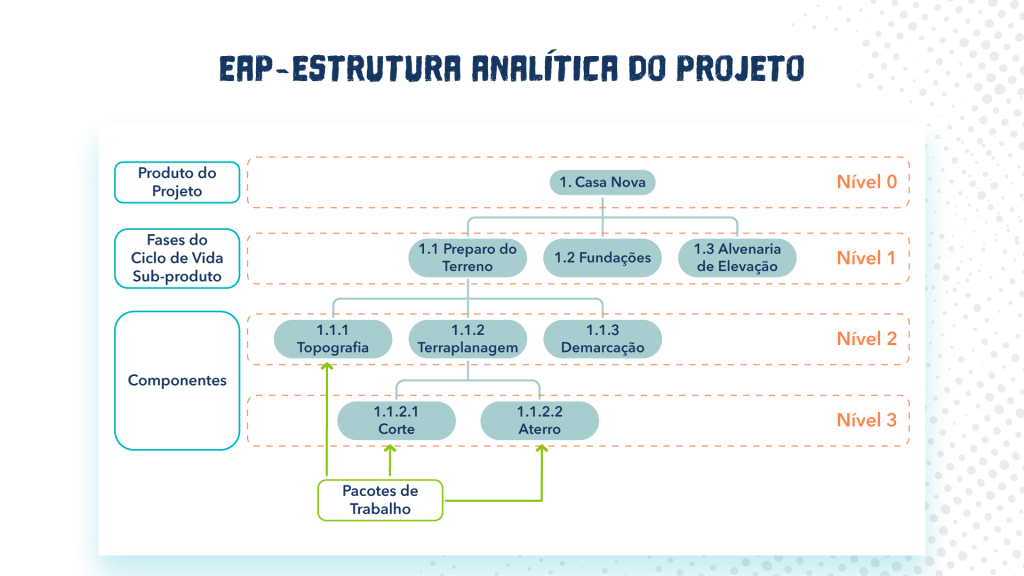
\includegraphics[width=0.7\linewidth]{dados/figuras/eap}
    \caption{EAP - Estrutura Analítica}
    \label{fig:eap}
\end{figure}

\section{Modelo de EAP}

Quando se trabalha com frequência num mesmo tipo de projeto, é possível evoluir a EAP e transformá-la num modelo. Isso tornará novos projetos muito mais rápidos, pois teremos um modelo de estrutura analítica de projeto, de cronograma, de estimativa de recursos e durações, tudo padronizado, algumas etapas economizadas, bastando uma adequação e revisão a cada projeto.

\section{Como montar o Dicionário da EAP (Estrutura Analítica do Projeto)}

O dicionário da EAP é uma tabela que descreve os pacotes de trabalho, seus responsáveis e critérios de aceitação. Essa ferramenta ajuda a complementar a estrutura analítica do projeto, pois traz informações que não puderam ser incluídas no diagrama da EAP. Dessa forma, ficam explícitas quais as expectativas em relação aos resultados das entregas do projeto.

Voltando ao nosso exemplo da casa, poderíamos ter o seguinte “verbete” no dicionário da EAP:

\begin{itemize}
\item Pacote de Trabalho: alvenaria de elevação
\item Descrição: levantamento de paredes, utilizando o método especificado no projeto de construção civil.
\item Responsável: Pedro Alcântara.
\item Participantes: Flávia Marcelino, Kássio Freitas.
\item Critérios de Aceitação: firmeza, ausência de rachaduras, bom isolamento térmico.
\end{itemize}

O dicionário da EAP é ótimo para ser consultado quando alguém fica com dúvidas a respeito daquilo que deve ser entregue, facilitando a comunicação do time. Além disso, também auxilia na hora de construir o cronograma, segundo passo depois da elaboração da EAP.
\nocite{eap}
                
%% REVISÃO DE LITERATURA--------------------------------------------------------

\chapter{REVISÃO DE LITERATURA}
\label{chap:fundamentacaoTeorica}

É uma boa prática iniciar cada novo capítulo com um breve texto introdutório (tipicamente, dois ou três parágrafos) que deve deixar claro o quê será discutido no capítulo, bem como a organização do capítulo.
Também servirá ao propósito de "amarrar"{} o conteúdo deste capítulo com o conteúdo do capítulo imediatamente anterior.
   % Revisão de Literatura
%% METODOLOGIA------------------------------------------------------------------

\chapter{METODOLOGIA}
\label{chap:metodologia}
Cada capítulo deve conter uma pequena introdução (tipicamente, um ou dois parágrafos) que deve deixar claro o objetivo e o que será discutido no capítulo, bem como a organização do capítulo.

\section{DELINEAMENTO DA PESQUISA}
\label{sec:titSecDelPesq}

Inserir seu texto aqui...

\section{COLETA E TRATAMENTO DE DADOS}
\label{sec:titSecColDad}

Inserir seu texto aqui...
             % Metodologia
%% RESULTADOS-------------------------------------------------------------------

\chapter{ANÁLISE E DISCUSSÃO DOS RESULTADOS}

Cada capítulo deve conter uma pequena introdução (tipicamente, um ou dois parágrafos) que deve deixar claro o objetivo e o que será discutido no capítulo, bem como a organização do capítulo.
              % Resultados
%% ORIENTAÇÕES GERAIS------------------------------------------------------------


% SOBRE AS ILUSTRAÇÕES----------------------------------------------------------
\chapter{SOBRE AS ILUSTRAÇÕES}
\label{chap:apSobreIlust}

A seguir exemplifica-se como inserir ilustrações no corpo do trabalho. As ilustrações serão indexadas automaticamente em suas respectivas listas. A numeração sequencial de figuras, tabelas e equações também ocorre de modo automático.

Referências cruzadas são obtidas através dos comandos \verb|\label{}| e \verb|\ref{}|. Sendo assim, não é necessário por exemplo, saber que o número de certo capítulo é \ref{chap:fundamentacaoTeorica} para colocar o seu número no texto. Outra forma que pode ser utilizada é esta: \autoref{chap:fundamentacaoTeorica}, facilitando a inserção, remoção e manejo de elementos numerados no texto sem a necessidade de renumerar todos esses elementos.

% FIGURAS-----------------------------------------------------------------------
\chapter{FIGURAS}
\label{chap:figuras}

Exemplo de como inserir uma figura. A \autoref{fig:figura-exemplo-1} aparece automaticamente na lista de figuras. Para saber mais sobre o uso de imagens no \LaTeX{} consulte literatura especializada \cite{Goossens2007}.

Os arquivos das figuras devem ser armazenados no diretório de "/dados".

\begin{figure}[!htb]
    \centering
    \sbox0{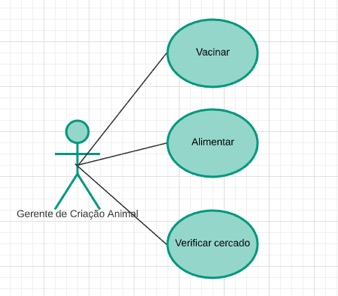
\includegraphics[width=0.5\textwidth]{./dados/figuras/figura1}}% measure width
    \begin{minipage}{\wd0}
    \usebox0
        \caption{Exemplo de Figura}
        \label{fig:figura-exemplo-1}
        \fonte{\citeonline{IRL2014}}
    \end{minipage}
\end{figure}

\begin{figure}[!htb]
    \centering
    \sbox0{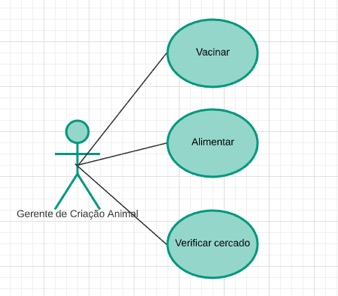
\includegraphics[width=0.5\textwidth]{./dados/figuras/figura1}}% measure width
    \begin{minipage}{\wd0}
    \usebox0
        \caption{Exemplo de Figura}
        \label{fig:figura-exemplo-2}
        \fonte{\citeonline{IRL2014}}
    \end{minipage}
\end{figure}

A \autoref{fig:figura-exemplo-1} Lorem Ipsum is simply dummy text of the printing and typesetting industry.
A \autoref{fig:figura-exemplo-2} Lorem Ipsum has been the industry's standard dummy text ever since the 1500s,
when an unknown printer took a galley of type and scrambled it to make a type
specimen book. It has survived not only five centuries, but also the leap into
electronic typesetting, remaining essentially unchanged. It was popularised in
the 1960s with the release of Letraset sheets containing Lorem Ipsum passages,
and more recently with desktop publishing software like Aldus PageMaker
including versions of Lorem Ipsum.

\begin{figure}[!htb]
    \sbox0{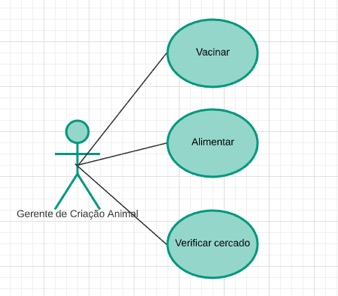
\includegraphics[width=0.5\textwidth]{./dados/figuras/figura1}}% measure width
    \begin{minipage}{\wd0}
    \usebox0
        \caption{Exemplo de Figura}
        \fonte{\citeonline{IRL2014}}
    \end{minipage}
    \label{fig:figura-exemplo1}
\end{figure}

% QUADROS E TABELAS---------------------------------------------------------------
\chapter{QUADROS E TABELAS}
\label{chap:tabelas}

Exemplo de como inserir o \autoref{qua:quadro-exemplo1} e a \autoref{tab:tabela-exemplo1}. Ambos aparecem automaticamente nas suas respectivas listas. Para saber mais informações sobre a construção de tabelas no \LaTeX{} consulte literatura especializada \cite{Mittelbach2004}.

Ambos os elementos (Quadros e Tabelas) devem ser criados em arquivos separados para facilitar manutenção e armazenados no diretório de "/dados".

\begin{quadro}[!htb]
    \centering
    \begin{tabular}{|p{7.5cm}|p{7.5cm}|}
        \hline
        \textbf{BD Relacionais} & \textbf{BD Orientados a Objetos} \\
        \hline
        Os dados são passivos, ou seja, certas operações limitadas podem ser automaticamente acionadas quando os dados são usados. Os dados são ativos, ou seja, as solicitações fazem com que os objetos executem seus métodos. & Os processos que usam dados mudam constantemente. \\
        \hline
    \end{tabular}
    \caption{Exemplo de Quadro.\label{qua:quadro-exemplo1}}
    \fonte{\citeonline{Barbosa2004}}
\end{quadro}


A diferença entre quadro e tabela está no fato que um quadro é formado por linhas horizontais e verticais. Deve ser utilizado quando o conteúdo é majoritariamente não-numérico. O número do quadro e o título vem acima do quadro, e a fonte, deve vir abaixo. E Uma tabela é formada apenas por linhas verticais. Deve ser utilizada quando o conteúdo é majoritariamente numérico. O número da tabela e o título vem acima da tabela, e a fonte, deve vir abaixo, tal como no quadro.

\begin{table}[!htb]
    \centering
    \begin{tabularx}{\textwidth}{rrrrr}
        \toprule
            & Valores 1 & Valores 2 & Valores 3 & Valores 4 \\
        \midrule
            Caso 1 & 0,86 & 0,77 & 0,81 & 163 \\
            Caso 2 & 0,19 & 0,74 & 0,25 & 180 \\
            Caso 3 & 1,00 & 1,00 & 1,00 & 170 \\
        \bottomrule
    \end{tabularx}
    \caption[Resultado dos testes]{Resultado dos testes.\label{tab:tabela-exemplo1}}
    \fonte{\citeonline{Barbosa2004}}
\end{table}


% EQUAÇÕES-----------------------------------------------------------------------
\chapter{EQUAÇÕES}
\label{chap:equacoes}

Exemplo de como inserir a \autoref{eq:equacao-exemplo1} e a Eq. \ref{eq:equacao-exemplo2} no corpo do texto \footnote{Deve-se atentar ao fato de a formatação das equações ficar muito boa esteticamente.}. Observe que foram utilizadas duas formas distintas para referenciar as equações.

\begin{equation}
    X(s) = \int\limits_{t = -\infty}^{\infty} x(t) \, \text{e}^{-st} \, dt
    \label{eq:equacao-exemplo1}
\end{equation}

\begin{equation}
    F(u, v) = \sum_{m = 0}^{M - 1} \sum_{n = 0}^{N - 1} f(m, n) \exp \left[ -j 2 \pi \left( \frac{u m}{M} + \frac{v n}{N} \right) \right]
    \label{eq:equacao-exemplo2}
\end{equation}

% ALGORITMOS-----------------------------------------------------------------------
\chapter{ALGORITMOS}
\label{chap:algoritmos}

Exemplo de como inserir um algoritmo. Para inserção de algoritmos utiliza-se o pacote {\ttfamily algorithm2e} que já está devidamente configurado dentro do template.

Os algoritmos devem ser criados em arquivos separados para facilitar manutenção e armazenados no diretório de "/dados".\\
\\

\begin{algorithm}
    \caption{Exemplo de Algoritmo}
    \KwIn{o número $n$ de vértices a remover, grafo original $G(V, E)$}
    \KwOut{grafo reduzido $G'(V,E)$}
    $removidos \leftarrow 0$ \\
    \While {removidos $<$ n } {
        $v \leftarrow$ Random$(1, ..., k) \in V$ \\
            \For {$u \in adjacentes(v)$} {
                remove aresta (u, v)\\
                $removidos \leftarrow removidos + 1$\\
            }
            \If {há  componentes desconectados} {
                remove os componentes desconectados\\
            }
        }
\end{algorithm}


% SOBRE AS LISTAS--------------------------------------------------------------------
\chapter{SOBRE AS LISTAS}
\label{chap:apSobreLista}

Para construir listas de "\textit{bullets}"{} ou listas enumeradas, inclusive listas aninhadas, é utilizado o pacote \verb|paralist|.

Exemplo de duas listas não numeradas aninhadas, utilizando o comando \verb|\itemize|. Observe a indentação, bem como a mudança automática do tipo de "\textit{bullet}"{} nas listas aninhadas.

\begin{itemize}
    \item item não numerado 1
    \item item não numerado 2
    \begin{itemize}
        \item subitem não numerado 1
        \item subitem não numerado 2
        \item subitem não numerado 3
    \end{itemize}
    \item item não numerado 3
\end{itemize}

Exemplo de duas listas numeradas aninhadas, utilizando o comando \verb|\enumerate|. Observe a numeração progressiva e indentação das listas aninhadas.

\begin{enumerate}
    \item item numerado 1
    \item item numerado 2
    \begin{enumerate}
        \item subitem numerado 1
        \item subitem numerado 2
        \item subitem numerado 3
    \end{enumerate}
    \item item numerado 3
\end{enumerate}

% SOBRE AS CITAÇÕES E CHAMADAS DE REFERÊNCAS----------------------------------------------
\chapter{SOBRE AS CITAÇÕES E CHAMADAS DE REFERÊNCAS}
\label{chap:apSobreCita}

Citações são trechos de texto ou informações obtidas de materiais consultadss quando da elaboração do trabalho. São utilizadas no texto com o propósito de esclarecer, completar e embasar as ideias do autor. Todas as publicações consultadas e utilizadas (por meio de citações) devem ser listadas, obrigatoriamente, nas referências bibliográficas, para preservar os direitos autorais. São classificadas em citações indiretas e diretas.

% CITAÇÕES INDIRETAS-----------------------------------------------------------------------
\chapter{CITAÇÕES INDIRETAS}
\label{chap:citacoesLivres}

É a transcrição, com suas próprias palavras, das idéias de um autor, mantendo-se o sentido original. A citação indireta é a maneira que o pesquisador tem de ler, compreender e gerar conhecimento a partir do conhecimento de outros autores. Quanto à chamada da referência, ela pode ser feita de duas maneiras distintas, conforme o nome do(s) autor(es) façam parte do seu texto ou não. Exemplo de chamada fazendo parte do texto:\\
\\Enquanto \citeonline{Maturana2003} defendem uma epistemologia baseada na biologia. Para os autores, é necessário rever \ldots.\\

A chamada de referência foi feita com o comando \verb|\citeonline{chave}|, que produzirá a formatação correta.

A segunda forma de fazer uma chamada de referência deve ser utilizada quando se quer evitar uma interrupção na sequência do texto, o que poderia, eventualmente, prejudicar a leitura. Assim, a citação é feita e imediatamente após a obra referenciada deve ser colocada entre parênteses. Porém, neste caso específico, o nome do autor deve vir em caixa alta, seguido do ano da publicação. Exemplo de chamada não fazendo parte do texto:\\
\\Há defensores da epistemologia baseada na biologia que argumentam em favor da necessidade de \ldots \cite{Maturana2003}.\\

Nesse caso a chamada de referência deve ser feita com o comando \verb|\cite{chave}|, que produzirá a formatação correta.

% CITAÇÕES DIRETAS-----------------------------------------------------------------------
\chapter{CITAÇÕES DIRETAS}
\label{chap:citacoesLiterais}

É a transcrição ou cópia de um parágrafo, de uma frase, de parte dela ou de uma expressão, usando exatamente as mesmas palavras adotadas pelo autor do trabalho consultado.

Quanto à chamada da referência, ela pode ser feita de qualquer das duas maneiras já mencionadas nas citações indiretas, conforme o nome do(s) autor(es) façam parte do texto ou não. Há duas maneiras distintas de se fazer uma citação direta, conforme o trecho citado seja longo ou curto.

Quando o trecho citado é longo (4 ou mais linhas) deve-se usar um parágrafo específico para a citação, na forma de um texto recuado (4 cm da margem esquerda), com tamanho de letra menor e espaçamento entrelinhas simples. Exemplo de citação longa:
\\\begin{citacao}
    Desse modo, opera-se uma ruptura decisiva entre a reflexividade filosófica, isto é a possibilidade do sujeito de pensar e de refletir, e a objetividade científica. Encontramo-nos num ponto em que o conhecimento científico está sem consciência. Sem consciência moral, sem consciência reflexiva e também subjetiva. Cada vez mais o desenvolvimento extraordinário do conhecimento científico vai tornar menos praticável a própria possibilidade de reflexão do sujeito sobre a sua pesquisa \cite[p.~28]{Silva2000}.
\end{citacao}

Para fazer a citação longa deve-se utilizar os seguintes comandos:
\begin{verbatim}
\begin{citacao}
<texto da citacao>
\end{citacao}
\end{verbatim}

No exemplo acima, para a chamada da referência o comando \verb|\cite[p.~28]{Silva2000}| foi utilizado, visto que os nomes dos autores não são parte do trecho citado. É necessário também indicar o número da página da obra citada que contém o trecho citado.

Quando o trecho citado é curto (3 ou menos linhas) ele deve inserido diretamente no texto entre aspas. Exemplos de citação curta:\\
\\A epistemologia baseada na biologia parte do princípio de que "assumo que não posso fazer referência a entidades independentes de mim para construir meu explicar" \cite[p.~35]{Maturana2003}.\\
\\A epistemologia baseada na biologia de \citeonline[p.~35]{Maturana2003} parte do princípio de que "assumo que não posso fazer referência a entidades independentes de mim para construir meu explicar".

% DETALHES SOBRE AS CHAMADAS DE REFERÊNCIAS---------------------------------------------------------
\chapter{DETALHES SOBRE AS CHAMADAS DE REFERÊNCIAS}
\label{chap:referUtilizadas}

Outros exemplos de comandos para as chamadas de referências e o resultado produzido por estes:\\
\\\citeonline{Maturana2003} \ \ \  \verb|\citeonline{Maturana2003}|\\
\citeonline{Barbosa2004} \ \ \   \verb|\citeonline{Barbosa2004}|\\
\cite[p.~28]{Silva2000} \ \ \  \verb|\cite[p.~28]{Silva2000}|\\
\citeonline[p.~33]{Silva2000} \ \ \   \verb|\citeonline[p.~33]{v}|\\
\cite[p.~35]{Maturana2003} \ \ \   \verb|\cite[p.~35]{Maturana2003}|\\
\citeonline[p.~35]{Maturana2003} \ \ \   \verb|\citeonline[p.~35]{Maturana2003}|\\
\cite{Barbosa2004,Maturana2003} \ \ \   \verb|\cite{Barbosa2004,Maturana2003}|\\

% SOBRE AS REFERÊNCIAS BIBLIOGRÁFICAS-------------------------------------------------------
\chapter{SOBRE AS REFERÊNCIAS BIBLIOGRÁFICAS}
\label{chap:apSobreRefer}

A bibliografia é feita no padrão \textsc{Bib}\TeX{}. As referências são colocadas em um arquivo separado. Neste template as referências são armazenadas no arquivo "base-referencias.bib".

Existem diversas categorias documentos e materiais componentes da bibliografia. A classe abn\TeX{} define as seguintes categorias (entradas):

\begin{verbatim}
@book
@inbook
@article
@phdthesis
@mastersthesis
@monography
@techreport
@manual
@proceedings
@inproceedings
@journalpart
@booklet
@patent
@unpublished
@misc
\end{verbatim}

Cada categoria (entrada) é formatada pelo pacote \citeonline{abnTeX22014d} de uma forma específica. Algumas entradas foram introduzidas especificamente para atender à norma \citeonline{NBR6023:2002}, são elas: \verb|@monography|, \verb|@journalpart|,\verb|@patent|. As demais entradas são padrão \textsc{Bib}\TeX{}. Para maiores detalhes, refira-se a \citeonline{abnTeX22014d}, \citeonline{abnTeX22014b}, \citeonline{abnTeX22014c}.

% NOTAS DE RODAPÉ--------------------------------------------------------------------------
\chapter{NOTAS DE RODAPÉ}
\label{chap:notasRodape}

As notas de rodapé pode ser classificadas em duas categorias: notas explicativas\footnote{é o tipo mais comum de notas que destacam, explicam e/ou complementam o que foi dito no corpo do texto, como esta nota de rodapé, por exemplo.} e notas de referências. A notas de referências, como o próprio nome ja indica, são utilizadas para colocar referências e/ou chamadas de referências sob certas condições.
             % Capítulo com Orientações de uso do Template
% CONCLUSÃO--------------------------------------------------------------------

\chapter{CONCLUSÃO}
\label{chap:conclusao}

Por meio do estudo durante o curso e das pesquisas realizadas para a elaboração do trabalho de Produção Textual Interdisciplinar Individual - PTI, houve um amadurecimento maior dos vários conceitos que serão empregados na carreira profissional, visto que  a inclusão crescente da tecnologia dentro das estratégias de negócio está levando todas as empresas a passarem por uma transformação digital — seja por enxergar as oportunidades que ela traz ou simplesmente por serem forçadas para se manterem competitivas.

No cenário proposto da empresa GlobalTecnol - Tecnologias, buscou-se o entendimento dos assuntos relativos a EAP, Sistemas Operacionais e segurança com a utilização de PenTest. E como a área de tecnologia da informação é muito dinâmica, o estudo para os itens mencionados e outros deve ser feito constante, para manter-se sempre atualizado com as nova tendências de mercado.
                 			         % Conclusão

\postextual
% INSERE ELEMENTOS PÓS-TEXTUAIS
% REFERÊNCIAS------------------------------------------------------------------

% Carrega o arquivo "base-referencias.bib" e extrai automaticamente as referências citadas

\bibliography{./base-referencias}
\bibliographystyle{abntex2-alf} % Define o estilo ABNT para formatar a lista de referências
% OBSERVAÇÕES------------------------------------------------------------------
% Este arquivo não precisa ser alterado.

           			   % Referências
% % APÊNDICES--------------------------------------------------------------------

\begin{apendicesenv}
\partapendices

% Primeiro apêndice------------------------------------------------------------
\chapter{Nome do apêndice} % Edite para alterar o título deste apêndice
\label{chap:apendiceA}

Lembre-se que a diferença entre apêndice e anexo diz respeito à autoria do texto e/ou material ali colocado.

Caso o material ou texto suplementar ou complementar seja de sua autoria, então ele deverá ser colocado como um apêndice. Porém, caso a autoria seja de terceiros, então o material ou texto deverá ser colocado como anexo.

Caso seja conveniente, podem ser criados outros apêndices para o seu trabalho acadêmico. Basta recortar e colar este trecho neste mesmo documento. Lembre-se de alterar o "label"{} do apêndice.

Não é aconselhável colocar tudo que é complementar em um único apêndice. Organize os apêndices de modo que, em cada um deles, haja um único tipo de conteúdo. Isso facilita a leitura e compreensão para o leitor do trabalho.

% Novo apêndice----------------------------------------------------------------
\chapter{Nome do outro apêndice}
\label{chap:apendiceB}

conteúdo do novo apêndice

\end{apendicesenv}
             			   % Apêndices
% % ANEXO------------------------------------------------------------------------

\begin{anexosenv}
\partanexos

% Primeiro anexo---------------------------------------------------------------
\chapter{Nome do anexo}     % edite para alterar o título deste anexo
\label{chap:anexoA}

Lembre-se que a diferença entre apêndice e anexo diz respeito à autoria do texto e/ou material ali colocado.

Caso o material ou texto suplementar ou complementar seja de sua autoria, então ele deverá ser colocado como um apêndice. Porém, caso a autoria seja de terceiros, então o material ou texto deverá ser colocado como anexo.

Caso seja conveniente, podem ser criados outros anexos para o seu trabalho acadêmico. Basta recortar e colar este trecho neste mesmo documento. Lembre-se de alterar o "label"{} do anexo.

Organize seus anexos de modo a que, em cada um deles, haja um único tipo de conteúdo. Isso facilita a leitura e compreensão para o leitor do trabalho. É para ele que você escreve.

% Novo anexo-------------------------------------------------------------------
\chapter{Nome do outro anexo}
\label{chap:anexoB}

conteúdo do outro anexo

\end{anexosenv}
               			   % Anexos

\end{document}
